\documentclass[border=5pt]{standalone}
\usepackage{tikz}
\usepackage{tikz-3dplot}
\usetikzlibrary{arrows.meta, 3d, perspective, calc}
\usepackage{amsmath}
\begin{document}
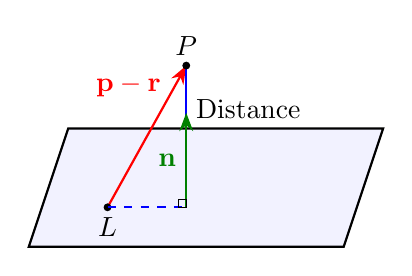
\begin{tikzpicture}[>=Stealth]
    % Plane
    \fill[blue!10, opacity=0.5] (0,0) -- (4,0) -- (4.5,1.5) -- (0.5,1.5) -- cycle;
    \draw[thick] (0,0) -- (4,0) -- (4.5,1.5) -- (0.5,1.5) -- cycle;

    % Line
    \draw[thick, red,->] (1,0.5) -- (2,2.3);
    \node[below left, red] at (1.8,2.3) {$\mathbf{p}-\mathbf{r}$};
    \draw[thick, blue] (2,2.3) -- (2,0.5);

    \node[above right] at (2,1.5) {Distance};

    \fill (2,2.3) circle (0.5mm);
    \node[above] at (2,2.3) {$P$};
    \fill (1,0.5) circle (0.5mm);
    \node[below] at (1,0.5) {$L$};

    % Normal vector
    \draw[->, thick, green!50!black] (2,0.5) -- node[left] {$\mathbf{n}$} (2,1.7);

    \draw[thick, dashed, blue] (1,0.5) -- (2,0.5);
    \draw (1.9,0.5) -- (2,0.5)--(2,0.6)--(1.9,0.6)--cycle;

\end{tikzpicture}
\end{document}
